% !TEX root = 00_main.tex
% TLDR: A reported judge--human correlation is a measurement to audit; the audit changes what it supports.
\section{Introduction}
\label{sec:intro}
% CS197 move 1: problem motivation -- proofs can succeed while required properties are missing; coverage needs a judge.
A Lean file can compile, and even prove every theorem it states, while omitting properties that its source program must satisfy.
Benchmarks that ask coding agents to formalize programs therefore score \emph{formal specification coverage}.
It measures how fully the agent's theorem statements express the obligations in a human-written reference.
% Provenance: public VeriBench report (TE1, theorem equivalence; SCSC product) and launch page ("Theorem coverage (TC1)").
\textsc{VeriBench} calls this quantity theorem equivalence (TE1) in its report and theorem coverage (TC1) on its launch page~\citep{veribench2026}.
Establishing coverage formally requires proving implications between statements, which is itself a hard proof task.
Such benchmarks delegate the coverage score to a language-model judge instead.
Because that score is one factor of the benchmark's multiplicative overall score~\citep{veribench2026}, the judge's agreement with expert judgment shapes what the benchmark measures.

% CS197 move 2: assumption -- one correlation with human ratings validates a judge.
Language-model judges are usually justified by their agreement with human ratings~\citep{zheng2023judging,liu2023geval,chiang2023can}.
That agreement is often summarized by a single correlation coefficient.
A correlation measures association rather than agreement: a method can correlate with a reference while reading consistently higher or lower~\citep{bland1986statistical}.
Its value also depends on choices that the coefficient does not record.
These include how ratings are grouped, which raters define the target, and whether the judge read the same inputs as the raters.

% CS197 move 3: contribution -- audit the reported number instead of accepting it.
We treat a reported judge--human correlation as a measurement to audit rather than a number to accept.
Our object is the evidence behind one benchmark launch claim.
\textsc{VeriBench} reports that a GPT-5.3-Codex judge given the raters' rubric reaches Pearson correlation $r=0.6137$ against its human ratings, with weaker rank correlations~\citep{veribench2026}.
It presents this result as an alignment check, not as evidence that its deployed coverage scorer was fitted to human ratings.
We ask what the reported number establishes about the judge.

% CS197 move 4: instantiation -- reanalysis of archived receipts with task resampling, absolute agreement, targets and an input check.
We reanalyze the archived per-artifact scores of that judge and the human ratings it was compared with, without new model calls or new ratings.
The data are 75 Lean artifacts from 25 tasks.
Five raters rated them on a 0--5 coverage rubric, and the judge scored each artifact three times.
We complement the reported coefficient with intervals that resample tasks and with rank and absolute agreement.
We also separate within-task from between-task correlation, vary the rater target, and hash-compare the judge's inputs with the rated files (Figure~\ref{fig:intervals}).

% CS197 move 5: evaluation -- headline numbers; POSTHOC_CLI_RUBRIC_JUDGE_AGREEMENT_11-12-2026.json.
The reported correlation reproduces exactly, but its 95\% interval over tasks is [0.213, 0.821], and Spearman correlation is 0.375 [0.013, 0.668].
The judge rates artifacts 0.825 points below the human mean on the 0--5 scale.
Its absolute-agreement intraclass correlation, 0.429, therefore falls well below its consistency intraclass correlation, 0.613.
After centering scores within each task, Pearson correlation drops to 0.358 [0.055, 0.635].
The Spearman correlation computed inside each task averages only 0.255 [$-0.073$, 0.579].
The same judge scores have Pearson correlation 0.702 with the mean of lenient raters and 0.372 with the mean of expert raters.
For eight of the 25 tasks, the judge's reference theorems differ from those the raters saw.
On the other 17 tasks, Spearman correlation is 0.565 [0.197, 0.800], but the downward offset remains.
A supervised isotonic remapping removes the offset but leaves Spearman correlation at 0.046, and its absolute error is close to that of a constant prediction.

% CS197 move 6: implications and contributions -- no verdict on validity from one coefficient; checklist.
These results neither validate nor reject the judge; they show that the reported coefficient alone cannot tell which.
They also concern a different judge from the one that produced the benchmark's reported coverage scores, which used another model and rubric~\citep{veribench2026}.
We make the following contributions:
\begin{enumerate}
\item We reconstruct the evidence behind a reported judge--human correlation for formal specification coverage and reproduce it exactly from archived receipts.
\item We show that task-level uncertainty, rank and absolute agreement, the choice of rater target, and mismatched judge inputs each change what the correlation supports, with task-bootstrap intervals for every statistic we derive against the pooled target.
\item We derive a short reporting checklist for audits of coverage judges from these findings.
\end{enumerate}

\begin{figure}[t]
\centering
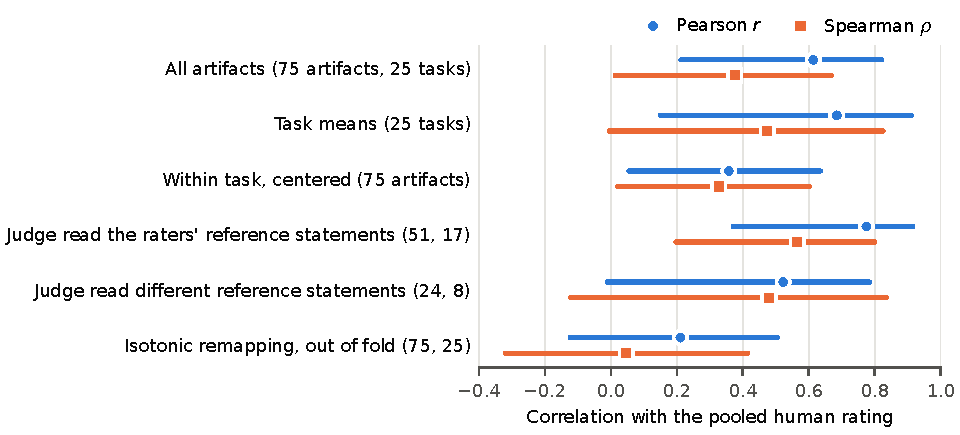
\includegraphics[width=\linewidth]{figures/agreement_intervals.pdf}
% Provenance: figures/make_agreement_figure.py reads POSTHOC_CLI_RUBRIC_JUDGE_AGREEMENT_11-12-2026.json; aggregates only.
\caption{\textbf{The same judge scores give correlations from near zero to 0.77, depending on how agreement is computed.} Pearson $r$ (circles) and Spearman $\rho$ (squares) between the GPT-5.3-Codex judge and the pooled human rating, with 95\% percentile intervals from 10,000 bootstrap draws over tasks.
Parentheses give artifacts and tasks.
The fourth and fifth rows split the artifacts by whether the judge read the same reference theorem statements as the raters (Section~\ref{sec:inputs}).
The last row applies an isotonic mapping fitted on the other fold of a two-fold task split.
Only the point estimates of the first and last rows appear in the original receipt; every interval and every other row is a post hoc analysis of the archived scores.}
\label{fig:intervals}
\end{figure}
